\documentclass[tikz,border=4pt]{standalone}
\usepackage{ctex}\usepackage{amsmath}
\usetikzlibrary{arrows.meta}
\begin{document}
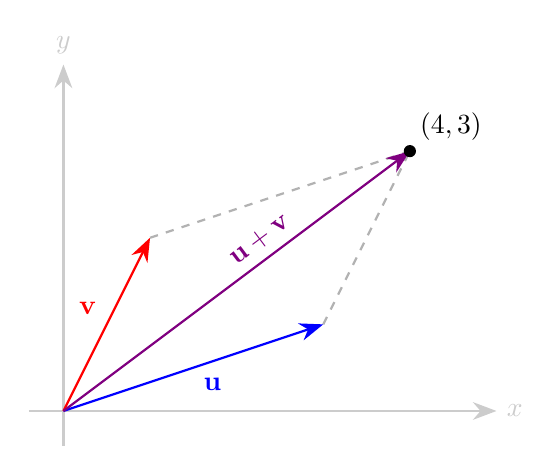
\begin{tikzpicture}[scale=1.1,>={Stealth[length=3mm]},thick]
  \draw[->,gray!40] (-0.4,0)--(5,0) node[right]{$x$};
  \draw[->,gray!40] (0,-0.4)--(0,4) node[above]{$y$};
  \draw[dashed,gray!60] (3,1)--(4,3);
  \draw[dashed,gray!60] (1,2)--(4,3);
  \draw[->,blue] (0,0)--(3,1) node[midway,below right]{$\mathbf{u}$};
  \draw[->,red] (0,0)--(1,2) node[midway,above left]{$\mathbf{v}$};
  \draw[->,violet] (0,0)--(4,3) node[pos=0.6,above,sloped]{$\mathbf{u}+\mathbf{v}$};
  \fill (4,3) circle(2pt) node[above right]{$(4,3)$};
\end{tikzpicture}
\end{document}
